\documentclass{article}
\usepackage[utf8]{inputenc}
\usepackage[english]{babel}
\usepackage{graphicx}

\title{Finding centroid of irregularly shaped 2D object}
\author{William Wang and Duy Nguyen}
\date{20 May 2016}

\begin{document}

\maketitle
\begin{abstract}
    In this paper, we investigate the method to balance an object. Using measurements from the real world, we used the magic of a calculator to regress the curved nature of the 2D object to a quartic equation. This enable us to apply the formula and find the center of mass of the object, and thus balance it. 
\end{abstract}
\section{Introduction}
    For this paper, we obtained a 2D object, which have three straight edges and one curve.
\section{Straight edges}
    The object was composed of four equation, three of which are stright lines. The equation for the straight line are presented thusly:
    
    $$ x = 0 $$
    $$ x = 20 $$
    $$ y = 0 $$
    
    The other non-linear equation is set to be approximate in the next section.
\section{Curve regression}
    To find the equation for the curve, we first need to gather some data of the curve. 
    
    The data obtained is presented in the appendix. Using this data and a TI-Nspire CX CAS, we obtained three different regression equation that could potentially matched the data.
    \begin{center}
    \textbf{Linear}
    $$ y = 0.01848x + 11.5381 $$
    $$ r^2 = 0.018848 $$
    \textbf{Quadratic}
    $$ y = -0.01959x^2 + 0.420201x + 10.1321 $$
    $$ r^2 = 0.582572 $$
    \textbf{Quartic}
    $$ y = 1.44\cdot10^{-4}x^4 - 0.002676335x^3 - 0.04064956x^2 + 0.879152x + 9.05122141$$
    $$ r^2 =  0.997008211 $$
    \end{center}
    
    Therefore, we chose the quartic equation for its high $r^2$ value.
    To make things clearer, we graphed these equations with the scatter plot of the data.
    \begin{center}
    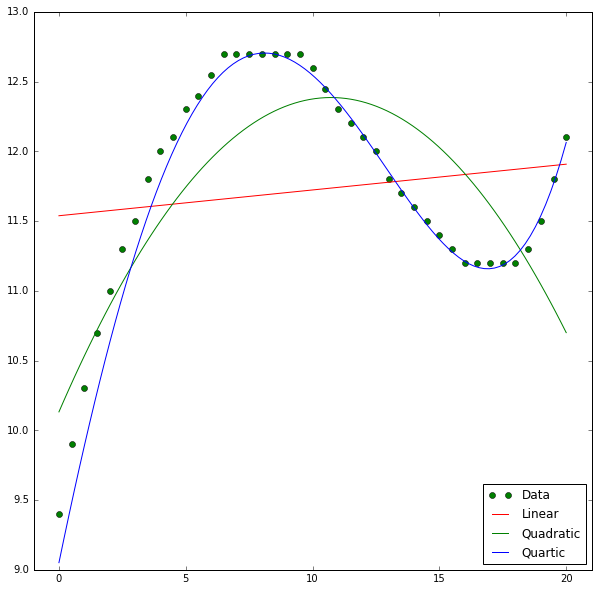
\includegraphics[width=10cm]{download}
    \end{center}
\section{Finding the center of mass}
    To find the center of mass, we must find the x-center ($\bar{x}$)and the y-center ($\bar{y}$) of the object.
    
    The equation we selected to use is the quartic equation. 
    $$ f(x) = 1.44\cdot10^{-4}x^4 - 0.002676335x^3 - 0.04064956x^2 + 0.879152x + 9.05122141$$
    
    First, we must find the area:
    $$Area = \int_{a}^{b} f(x) dx $$
    $$\int_{0}^{20} 1.44\cdot10^{-4}x^4 - 0.002676335x^3 - 0.04064956x^2 + 0.879152x + 9.05122141  dx $$
    $$Area = 233.801$$
    
    $$\bar{x} = \frac{1}{Area} \int_{a}^{b} xf(x) dx$$
    $$\bar{x} = 10.076 $$
    $$\bar{y} = \frac{1}{Area} \int_{a}^{b} \frac{1}{2} (f(x)^2 - g(x)^2) dx$$
    $$\bar{y} = 5.874 $$
    
    Therefore, the center of mass should be at \textbf{(10.076, 5.874)}.
    
    
\pagebreak    
\section{Appendix: Data table for the curve}
    Using graph paper and ruler, we have measured the curve as follow:
\begin{table}[ht]
\begin{minipage}[b]{0.45\linewidth}\centering
\begin{tabular}{c|c}
x (cm)	&	y (cm) \\ \hline
0	&	9.4 \\
0.5	&	9.9 \\
1	&	10.3 \\
1.5	&	10.7 \\
2	&	11 \\
2.5	&	11.3 \\
3	&	11.5 \\
3.5	&	11.8 \\
4	&	12 \\
4.5	&	12.1 \\
5	&	12.3 \\
5.5	&	12.4 \\
6	&	12.55 \\
6.5	&	12.7 \\
7	&	12.7 \\
7.5	&	12.7 \\
8	&	12.7 \\
8.5	&	12.7 \\
9	&	12.7 \\
9.5	&	12.7 \\
10	&	12.6 \\
    \end{tabular}
\end{minipage}
\hspace{0.5cm}
\begin{minipage}[b]{0.45\linewidth}
\centering
\begin{tabular}{c|c}
   x (cm)	&	y (cm) \\ \hline 
10.5	&	12.45 \\
11	&	12.3 \\
11.5	&	12.2 \\
12	&	12.1 \\
12.5	&	12 \\
13	&	11.8 \\
13.5	&	11.7 \\
14	&	11.6 \\
14.5	&	11.5 \\
15	&	11.4 \\
15.5	&	11.3 \\
16	&	11.2 \\
16.5	&	11.2 \\
17	&	11.2 \\
17.5	&	11.2 \\
18	&	11.2 \\
18.5	&	11.3 \\
19	&	11.5 \\
19.5	&	11.8 \\
20	&	12.1 \\
    \end{tabular}
\end{minipage}
\end{table}
\end{document}
